\section{Planar monotonicity}\label{sec:planar}
This section proves that in the plane the realised union is monotone under every inclusion of relation lattices and every box. The proof has three parts: a decomposition of cells into smaller cells of the target (\cref{sec:tools}), an exact criterion for when a cell can leave the target (\cref{sec:zero}), and the geometry of the cells that satisfy that criterion (\cref{sec:lg,sec:p5p1}). \Cref{sec:g12} places the result relative to the inherited planar stabilisation theorem.

\subsection{Two tools: conformal decomposition and zonotopal tiling}\label{sec:tools}
\begin{lemma}[conformal decomposition]\label{lem:L1}
Every $v$ in a lattice $M$ is a finite sum of Graver vectors of $M$, each conformally $\cm v$.
\end{lemma}
\prov{CW-0499}{E2P4v5-L1}{PROVED}{FULL}
\begin{proof}
Induction on $|v|_1$. For $v=0$ the sum is empty. Otherwise the set of nonzero lattice vectors $\cm v$ is finite and nonempty; a member $g$ of minimal $\ell_1$-norm is Graver (a nonzero $w'\cm g$ would also be $\cm v$ and shorter). Now $v-g\cm v$ is shorter; apply induction and transitivity of $\cm$. \qedhere
\end{proof}
\begin{lemma}[explicit tiling]\label{lem:T0}
Let $v_1,\dots,v_n$ be nonzero integer vectors spanning a $d$-dimensional subspace, written in lattice coordinates of the span, and $Z(V)=\sum[0,1]v_i$. Then $Z(V)$ is covered by finitely many tiles $T_S$, with pairwise disjoint interiors, each a translate of a parallelotope $Z(V_S)=\sum_{i\in S}[0,1]v_i$ with $V_S$ linearly independent, and every vertex of every tile is a subset sum $\sum_{i\in A}v_i$.
\end{lemma}
\prov{CW-0500}{E2P4v5-T0}{PROVED}{ADAPTED}
\begin{proof}
If $n=d$, $Z(V)$ is one parallelotope. Otherwise choose integer heights $w_i$ so generic that for every $d$-subset $S$ with $\det V_S\ne0$ and every $i\notin S$ the lifted vector $\tilde v_i=(v_i,w_i)\in\R^{d+1}$ is not in $\mathrm{span}(\tilde v_s:s\in S)$ (finitely many hyperplanes in $w$ are avoided: the coefficient of $w_i$ is $1$). For such $S$ let $\nu_S$ be a normal of $\mathrm{span}(\tilde v_S)$, signed with negative last coordinate (nonzero: it is $\pm\det V_S$), $A_S=\{i\notin S:\nu_S\cdot\tilde v_i>0\}$ and $T_S=\sum_{i\in A_S}v_i+Z(V_S)$. The face of the lifted zonotope $\tilde Z=\sum[0,1]\tilde v_i$ on which a functional $\nu$ is maximal is $\sum_{\nu\cdot\tilde v_i>0}\tilde v_i+\sum_{\nu\cdot\tilde v_i=0}[0,1]\tilde v_i$; by genericity the facets of $\tilde Z$ are the sets $\sum_{i\in A_S}\tilde v_i+Z(\tilde v_S)$, and such a facet is \emph{lower} iff $\nu_S$ has negative last coordinate. The lower facets project onto $T_S$ injectively, and \emph{by the lifting lemma (\cref{lem:lift})} they cover the shadow $Z(V)$ with disjoint interiors; (c) is the definition of $T_S$. \qedhere
\end{proof}
\noindent\textbf{The lifting fact.} The covering property used above is the standard statement that the lower facets of a lifted polytope project onto its shadow with disjoint interiors (the regular subdivision induced by a lifting, \cite{Ziegler1995,DLRS2010}; it is the construction behind the Bohne--Dress correspondence for zonotopal tilings \cite{Bohne1992,RGZ1994,HRS2000,BLSWZ1999}). It is proved in \cref{app:lifting} (\cref{lem:lift}), so \cref{lem:T0} is PROVED in full; the qualification of the first version is withdrawn. The release also checks the lemma numerically (volume sum $=\sum_S|\det V_S|$ and point location for random configurations), which is evidence for the implementation, not part of the proof.

\subsection{The zero-vertex criterion}\label{sec:zero}
Let $\Lambda\subseteq\Lambda'\subseteq\Z^k$ be lattices and $Q$ a box.
\begin{proposition}[zero-vertex criterion]\label{prop:Z}
Let $c=\Pil(u;g_1,\dots,g_j)$ be a cell of $\Kabs(\Lambda,Q)$, and call \emph{zero-vertex decomposition} a choice of $s_i\in\Lambda'$ with $s_i\cm g_i$ (possibly $0$ or $g_i$) and $u+\sum s_i=0$.
\begin{enumerate}[label=(Z.\arabic*)]
\item If $c$ has no zero-vertex decomposition then $c\subseteq U(\Lambda',Q)$.
\item $c$ has a zero-vertex decomposition iff $m(c):=u+\sum_ig_i^-=0$ and $g_i^-\in\Lambda'$ for all $i$ (then $s_i=g_i^-$).
\item Every cell has $2^j$ representations (base corner and generator signs), and Z.1 applies to each. Hence $c\subseteq U(\Lambda',Q)$ unless $m(c)=0$ and $g_i^-\in\Lambda'$ for all $i$ (equivalently $g_i^+\in\Lambda'$, since $g_i\in\Lambda\subseteq\Lambda'$). Cells with this property are \emph{hard}.
\item There are no hard cells of dimension $\le1$ (edges never obstruct).
\end{enumerate}
\end{proposition}
\prov{CW-0501}{E2P4v5-Z}{PROVED}{FULL}
\prov{CW-0490}{P4-Z1}{PROVED}{FULL}
\prov{CW-0496}{P4-Z2}{PROVED}{FULL}
\prov{CW-0491}{P4-Z1.a}{PROVED}{FULL}
\begin{proof}
(Z.1) By \cref{lem:L1} write each $g_i=\sum_th_{i,t}$ with $h_{i,t}\in\Gr(\Lambda')$ and $h_{i,t}\cm g_i$. Then $Z'=u+\sum_{i,t}[0,1]h_{i,t}$ contains $c$ (for $\lambda_i\in[0,1]$, $\lambda_ig_i=\sum_t\lambda_ih_{i,t}$). Tile $Z'$ by \cref{lem:T0}. A vertex of a tile is $u+\sum_{(i,t)\in A}h_{i,t}=u+\sum_is_i$, where $s_i$ is a partial sum of the pieces of $g_i$; all pieces have the sign pattern of $g_i$, so $s_i\in\Lambda'$ and $s_i\cm g_i$. For each coordinate $\ell$ the vertex coordinate lies between $u_\ell+\sum_i\min(g_{i,\ell},0)$ and $u_\ell+\sum_i\max(g_{i,\ell},0)$, which are coordinates of two corners of $c$, hence in $[0,q_\ell]$: the vertex is in $Q$. It is nonzero by hypothesis. So every tile (generators $h_{i,t}$ Graver in $\Lambda'$ and in the box, independent, all vertices in $F(\Lambda',Q)$) is a cell of $\Lambda'$, and $c\subseteq Z'\subseteq U(\Lambda',Q)$.

(Z.2) ($\Rightarrow$) Coordinatewise $s_{i,\ell}\ge\min(g_{i,\ell},0)$, so $0=u_\ell+\sum_is_{i,\ell}\ge m_\ell$; but $m_\ell$ is a coordinate of the corner $u+\sum_{g_{i,\ell}<0}g_i$ of $c$, hence $\ge0$. So equality holds throughout: $m=0$ and $s_{i,\ell}=\min(g_{i,\ell},0)$, that is $s_i=g_i^-\in\Lambda'$. ($\Leftarrow$) Take $s_i=g_i^-\cm g_i$.

(Z.3) $m(c)$ is the coordinatewise minimum of the corners, independent of the representation; the representation with generators $\epsilon_ig_i$ has outgoing negative parts $(\epsilon_ig_i)^-\in\{g_i^-,-g_i^+\}$. All $2^j$ representations have a zero-vertex decomposition iff $m(c)=0$ and both $g_i^-$ and $g_i^+$ lie in $\Lambda'$ for every $i$.

(Z.4) If a cell $\Pil(u;g)$ were hard then $u+g^-=0$, so $-u=g^-$, a nonzero element of $\Lambda$ ($u\in F\subseteq\Lambda$) with $g^-\cm g$; and $g^-\ne g$, else $u+g=0\notin F$. This contradicts $g\in\Gr(\Lambda)$. Points are covered trivially. \qedhere
\end{proof}
The release gives (Z.1) and (Z.2) first as P4-Z1, P4-Z2 and then re-proves them with a complete argument as Z; the three records are merged here with one proof.

\subsection{Adjacent corners overlap in support}\label{sec:lg}
\begin{lemma}\label{lem:LG}
If $P,P'$ are corners of a cell of $U(\Lambda,Q)$ that differ by one generator $w=P'-P$, then $\supp P\cap\supp P'\ne\emptyset$.
\end{lemma}
\prov{CW-0502}{E2P4v5-LG}{PROVED}{FULL}
\begin{proof}
$P,P'$ are nonzero and $\ge0$. If the supports were disjoint then $P'\cm w$ and $-P\cm w$ (on $\supp P'$, $w_\ell=P'_\ell\ge0=P_\ell$; on $\supp P$, $w_\ell=-P_\ell\le0=P'_\ell$; zero elsewhere), both lie in $\Lambda$ and are nonzero, $P'\ne w$ (else $P=0$) and $-P\ne w$ (else $P'=0$): $w$ would not be Graver. \qedhere
\end{proof}

\subsection{The planar theorem}\label{sec:p5p1}
\begin{theorem}[planar monotonicity]\label{thm:planar}
Let $\Lambda\subseteq\Lambda'\subseteq\Z^2$ be lattices of rank $2$ and $Q=[0,a]\times[0,b]$ any box. Then $U(\Lambda,Q)\subseteq U(\Lambda',Q)$.
\end{theorem}
\prov{CW-0504}{P5-P1}{PROVED}{FULL}
\prov{CW-0497}{P4-P1}{PROVED}{FULL}
\begin{proof}
Points are trivial and edges are covered by \cref{prop:Z}(Z.4) and (Z.3). Let $c$ be a $2$-cell. If it is not hard, \cref{prop:Z}(Z.3) applies. Let it be hard. Let $k',l'\ge1$ be minimal with $k'e_1,l'e_2\in\Lambda'$ (they exist: finite index), so $\{t:te_1\in\Lambda'\}=k'\Z$. Then $k'e_1$ and $l'e_2$ are Graver in $\Lambda'$: a nonzero conformal subvector of $k'e_1$ in $\Lambda'$ is $(t,0)$ with $0<t\le k'$, so $t=k'$.
\begin{enumerate}[label=(\arabic*),leftmargin=*]
\item $m(c)=0$ gives a corner $A$ with $x=0$ and a corner $B$ with $y=0$; both are nonzero, so $A=(0,y_0)$, $B=(x_0,0)$ with $x_0,y_0>0$.
\item $\supp A=\{2\}$ and $\supp B=\{1\}$ are disjoint, so by \cref{lem:LG} $A,B$ are not adjacent: they are opposite corners. Let $D,E$ be the other two.
\item Write the edge vectors at $A$ as $g',h'$ with $B=A+g'+h'$, $D=A+g'$, $E=A+h'$. Since $D,E\in Q$: $g'_1,h'_1\ge0$ and $y_0+g'_2,y_0+h'_2\ge0$. As $g'_2+h'_2=-y_0$, both $g'_2,h'_2\le0$. Write $g'=(g_1,-g_2)$, $h'=(h_1,-h_2)$ with $g_1,g_2,h_1,h_2\ge0$, $g_1+h_1=x_0$, $g_2+h_2=y_0$; then $D=(g_1,h_2)$, $E=(h_1,g_2)$.
\item All four numbers are positive: $D$ is adjacent to both $A$ and $B$ and nonzero, so by \cref{lem:LG} $\supp D$ meets $\{2\}$ and $\{1\}$: $h_2>0$ and $g_1>0$. Likewise for $E$: $h_1>0$, $g_2>0$.
\item Hardness: $g'^{+}=(g_1,0)$, $g'^-=(0,-g_2)$, $h'^+=(h_1,0)$, $h'^-=(0,-h_2)$ lie in $\Lambda'$ (up to the sign convention of \cref{prop:Z}(Z.3)). Hence $k'\mid g_1,h_1$ and $l'\mid g_2,h_2$, so $g_1,h_1\ge k'$ and $g_2,h_2\ge l'$; $x_0=g_1+h_1\in k'\Z$, $x_0\ge2k'$, $y_0\in l'\Z$, $y_0\ge2l'$.
\item The four corners satisfy $x/k'+y/l'\ge2$ ($A$: $y_0/l'\ge2$; $B$: $x_0/k'\ge2$; $D$: $g_1/k'+h_2/l'\ge2$; $E$ likewise). By convexity every $p\in c$ has $p_1/k'+p_2/l'\ge2$, so \textbf{$p_1\ge k'$ or $p_2\ge l'$}.
\item The rectangles $R_{ij}=[ik',(i+1)k']\times[jl',(j+1)l']$, $0\le i<x_0/k'$, $0\le j<y_0/l'$, tile $[0,x_0]\times[0,y_0]\subseteq Q$ (the box contains the bounding box of the corners). Their corners lie in $k'\Z\times l'\Z\subseteq\Lambda'$, in $Q$, and are nonzero except the corner $0$ of $R_{00}$. So each $R_{ij}$, $(i,j)\ne(0,0)$, is the cell $\Pil(\text{corner};k'e_1,l'e_2)$ of $U(\Lambda',Q)$. A point $p\in c$ with $p_1\ge k'$ lies in some $R_{ij}$ with $i\ge1$ (because $x_0/k'\ge2$), and one with $p_2\ge l'$ lies in some $R_{ij}$ with $j\ge1$. Hence $c\subseteq U(\Lambda',Q)$. \qedhere
\end{enumerate}
\end{proof}
\begin{figure}[tbp]\centering
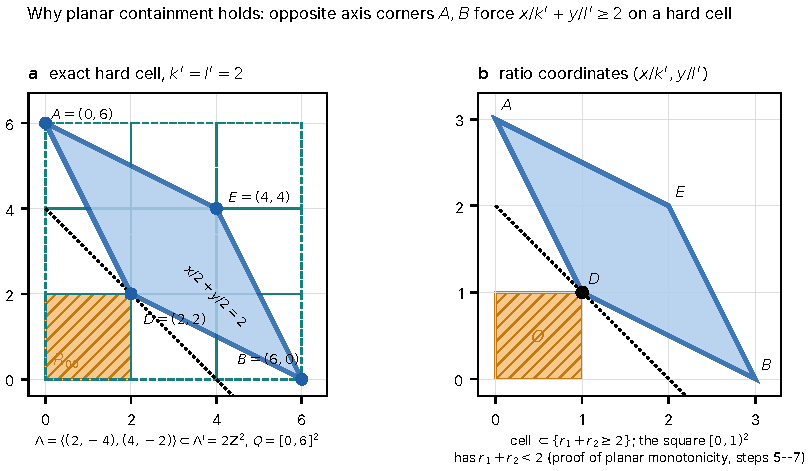
\includegraphics[width=0.98\textwidth]{fig08_planar_proof}
\caption{Geometry of the planar proof (\cref{thm:planar}, steps (1)--(7); \emph{exact computation of one instance of the construction}). Hard cell $c=\Pil((0,6);(2,-4),(4,-2))$ of the source lattice $\{x+2y\equiv0,\ 2x+y\equiv0\ (6)\}$, target $\Lambda'=2\Z^2$ (so $k'=l'=2$), box $[0,6]^2$. (a)~Opposite axis corners $A=(0,6)$ and $B=(6,0)$ and the other two corners $D=(2,2)$, $E=(4,4)$; the dotted line $x/k'+y/l'=2$ (i.e.\ $x+y=4$) passes through $D$, the corners $A,B,E$ lie strictly above it, and the whole cell lies on or above it; the $2\times2$ rectangles of the target tiling of $[0,x_0]\times[0,y_0]$ are dashed teal, and the corner square $[0,2]^2$ at the origin (orange, hatched) is the region the cell never enters. (b)~The same cell in the ratio coordinates $(x/k',y/l')$, where all four corners satisfy the inequality; by convexity so does every point of $c$. All $441$ grid points of $c$ were tested exactly against $U(2\Z^2,Q)$. The cell is an actual hard cell, not a schematic; the picture illustrates the general argument by this instance.}\label{fig:planarproof}
\end{figure}
\begin{remark}[why the plane works]\label{rem:whyplane}
In the proof the cell escapes only through the origin, and the escape is blocked by a fact that is special to $k=2$: opposite axis corners $A=(0,y_0)$, $B=(x_0,0)$ force every point of the cell to satisfy $x/k'+y/l'\ge2$, and for two ratios ``sum $\ge2$'' implies ``one ratio $\ge1$''. For three ratios a sum of $2$ is compatible with all ratios $<1$: in \cref{thm:C1} the failing cell has all four corners at ratio sum exactly $2$ (with axis orders $(2,2,2)$), and its point $(\tfrac23,\tfrac53,\tfrac53)$ has ratios $(\tfrac13,\tfrac56,\tfrac56)$, all $<1$. This explains where the planar argument cannot be repeated; it is not by itself a theorem about dimension three, and the failures proved in \cref{sec:obstruction} do not depend on it.
\end{remark}
\begin{corollary}[earlier planar conjectures]\label{cor:CP}
Conjecture CP2 (planar containment for $\Lambda\subsetneq\Lambda'$, same primes and box) and conjecture CP3-A (residual planar containment) of the earlier releases are theorems for nested lattices: they are \cref{thm:planar}. Both records remain in the crosswalk with their historical status OPEN; they are not restated.
\end{corollary}
\prov{CW-0473}{CP2}{OPEN}{EXCLUDED}
\prov{CW-0482}{CP3-A}{OPEN}{EXCLUDED}

\subsection{Relation to the inherited planar stabilisation theorem}\label{sec:g12}
GEO-I (v004 S1, cited as \texttt{CW-0477}) reduces every planar lattice $\Lambda_b$ to a normal form $\mathrm{diag}(a,c)\,\Gamma_{d,s}$ with $\Gamma_{d,s}=\{(i,j):j\equiv si\ (\mathrm{mod}\ d)\}$, $s$ a unit, and box $(\lfloor q_1/a\rfloor,\lfloor q_2/c\rfloor)$. The inherited theorem G12-T8 (GEO-I v012; cited as \texttt{CW-0478}, not reproved) states: for $d\ge2$, normalised box $\ge(d,d)$ and $\ne(d,d)$ one has $U=\conv F$. In that regime $U\subseteq U'$ follows from $F\subseteq F'$ by \cref{lem:gap} with no hypothesis on the lattices. \Cref{thm:planar} complements this: it needs $\Lambda\subseteq\Lambda'$ but holds for \emph{every} box, including the exceptional hollow box $(d,d)$ and sub-threshold boxes, where $U\ne\conv F$. The planar hole creation and destruction of \cref{prop:topology} occurs exactly at those exceptional boxes (ER-19).
\prov{CW-0477}{P3-L1}{PROVED}{CITED}
\prov{CW-0478}{P3-C1}{PROVED}{CITED}

\subsection{Scope for collective transitions}\label{sec:p5p1a}
\begin{proposition}[scope of the FIELD-I corollary (ER-23)]\label{prop:scope}
Let $x\to\Cmap(x)$ be an admissible planar transition ($k=2$, same primes and box). Then $U(\Lambda_x,Q)\subseteq U(\Lambda_{\Cmap(x)},Q)$ \emph{provided} $\Lambda_x\subseteq\Lambda_{\Cmap(x)}$. The collective map guarantees only $F\subseteq F'$, and lattices that shrink or are incomparable do occur (\cref{prop:corpus}), so \cref{thm:planar} does not by itself settle every planar transition.
\end{proposition}
\prov{CW-0505}{P5-P1.a}{PROVED}{FULL}
\begin{proof}
The first sentence is \cref{thm:planar}; the rest restates \cref{prop:fibre-vs-lattice}(b) and \cref{prop:corpus}. \qedhere
\end{proof}
For a transition with $F\subseteq F'$ but incomparable lattices, containment of the unions is not established in this manuscript.
